\appendix

\section{Oracle Accuracy-Utility Analysis}
\label{app:oracle}

We stratify SWE-bench Verified instances by F2P test count $T$, comparing per-test vs.\ trajectory-level oracle resolve rates under i.i.d.\ and block-correlated error models (ICC $= 0.191$, from function-level TOST analysis; \S\ref{sec:equivalence}).

\begin{table}[h]
\centering
\small
\caption{Oracle accuracy-utility frontier: per-test advantage stratified by F2P test count ($T$) on SWE-bench Verified (500 instances). Block-correlated model uses function-level ICC $= 0.191$ (from TOST equivalence analysis). P2P regression rate: 1.04\% mean, 0\% median.}
\label{tab:oracle}
\resizebox{\columnwidth}{!}{%
\setlength{\tabcolsep}{3pt}
\begin{tabular}{lcccc}
\toprule
\textbf{$T$} & \textbf{Inst.\%} & \textbf{i.i.d.\ (\pp{})} & \textbf{Block (\pp{})} & \textbf{Contrib.\%} \\
\midrule
$1$ & 68.7 & $-$0.04 & $-$0.09 & $\approx$0 \\
$2$ & 19.1 & 18.49 & 31.69 & 55.3 \\
$3$--$5$ & 7.1 & 25.00 & 40.74 & $\approx$26 \\
$\geq 6$ & 5.1 & 30.00 & 40.06 & $\approx$19 \\
\midrule
\textbf{All} & 100.0 & --- & \textbf{10.93} & 100.0 \\
\bottomrule
\end{tabular}}
\end{table}

\begin{figure}[h]
\centering
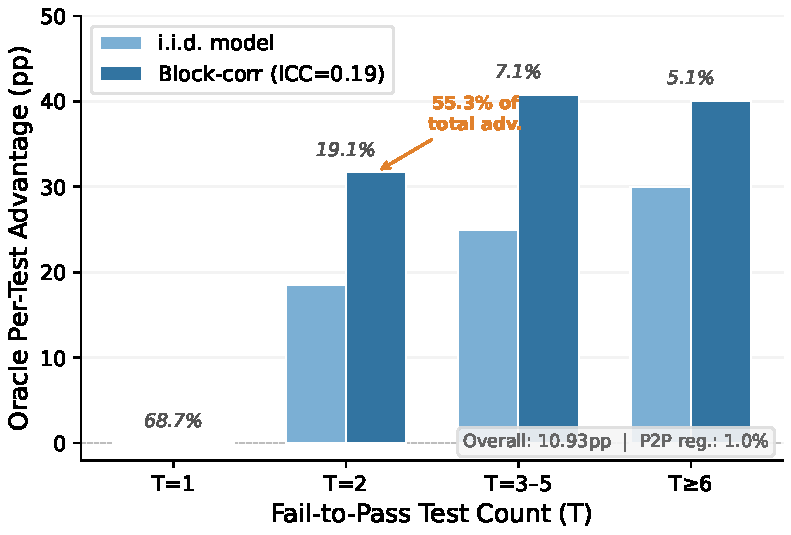
\includegraphics[width=\columnwidth]{figures/paper/fig3_oracle_stratified.pdf}
\caption{Oracle per-test advantage by F2P test count $T$. Advantage is zero at $T{=}1$ (68.7\%) and concentrates at $T{=}2$ (19.1\%, contributing 55.3\% of total advantage).}
\label{fig:oracle_stratified}
\end{figure}

Table~\ref{tab:oracle} and Figure~\ref{fig:oracle_stratified} reveal a sharp concentration: at $T = 1$ (68.7\% of instances), per-test and trajectory-level are informationally equivalent. The advantage materializes at $T = 2$ (19.1\%), where block-correlated advantage reaches 31.69\pp{} (55.3\% of total). The overall block-correlated advantage is 10.93\pp{}, driven by the $T \geq 2$ minority. Block correlation amplifies relative to i.i.d.: at $T = 2$, 31.69\pp{} vs.\ 18.49\pp{} (1.7$\times$). P2P regression is negligible (1.04\% mean, 0\% median); the practical value concentrates in F2P discrimination.

\paragraph{Sensitivity to ICC estimate.}
The analysis above uses ICC $= 0.191$ from function-level TOST equivalence testing (\S\ref{sec:equivalence}), where mean cluster size $\bar{k} \approx 16.5$ yields DEFF $= 3.97$. At repository level, within-problem correlation is substantially stronger: ICC $= 0.3146$ with DEFF $= 114.4$ (\S\ref{sec:repo}), reflecting the larger and more heterogeneous test suites in SWE-bench Verified problems. Under higher ICC, within-problem errors cluster more tightly, amplifying the block-correlated per-test advantage at each $T$ stratum---the correction from i.i.d.\ to block-correlated grows monotonically with ICC. The function-level ICC $= 0.191$ used in Table~\ref{tab:oracle} thus provides a conservative lower bound on the per-test advantage; the repo-level correlation structure would yield an even larger gap between per-test and trajectory-level oracle resolve rates, strengthening the case for per-test granularity at repository-level complexity.

\section{Ablation Studies}
\label{app:ablations}

\paragraph{LoRA rank sensitivity.}
All \cwm{} experiments use LoRA rank $r{=}16$. To test whether this capacity constraint handicaps \cwm{}, we train rank-32 variants (seed 42), doubling adapter parameters.

\begin{table}[h]
\centering
\small
\caption{LoRA rank ablation for \cwm{} 4B (seed 42, 3 epochs, lr $= 2{\times}10^{-4}$). Rank-16 seed variance: 0.53\pp{} (seeds 42 vs.\ 456).}
\label{tab:rank_ablation}
\setlength{\tabcolsep}{4pt}
\begin{tabular}{lccccc}
\toprule
\textbf{Config} & \textbf{$\alpha/r$} & \textbf{Acc (\%)} & \textbf{Fail \fone{}} & \textbf{Pass \fone{}} & \textbf{$\Delta$} \\
\midrule
$r{=}16$, $\alpha{=}32$ & 2 & \textbf{87.51} & --- & --- & --- \\
$r{=}32$, $\alpha{=}32$ & 1 & 87.00 & 87.1 & 86.9 & $-$0.51 \\
$r{=}32$, $\alpha{=}64$ & 2 & 87.04 & 87.27 & 86.79 & $-$0.47 \\
\bottomrule
\end{tabular}
\end{table}

Both rank-32 variants fall within the 2-seed variance of the rank-16 baseline (0.53\pp{} between seeds 42 and 456). The $\alpha{=}64$ variant (matching the baseline $\alpha/r{=}2$ ratio) rules out the confound that the $\alpha{=}32$ result might reflect reduced effective scaling rather than rank insensitivity. This is consistent with \cwm{}'s function-level performance being bounded by output-format constraints rather than adapter capacity.

\paragraph{Majority voting.}
Majority voting ($K{=}3$) decreases accuracy from 87.51\% to 86.83\% ($-$0.68\pp{}): errors are systematic rather than stochastic, so sampling-based ensembles do not help.

\paragraph{Sequence-length ablation details.}
Both formulations are trained with \texttt{max\_seq\_length}$=$2,048. At inference, \cwm{} reserves \texttt{max\_new\_tokens}$=$1,024, leaving ${\sim}$1,024 effective input tokens; \cls{} allocates nearly all context to input (5,120--8,192 tokens). A matched-context ablation (\cls{} 8B at 2,048 tokens) achieves 83.04\%, only 1.44\pp{} below the 8,192-token evaluation (84.48\%), though truncation introduces 136 unparseable outputs (1.39\% of test samples). The matched-context gap (\cls{}@2,048 vs.\ \cwm{}@2,048) is 25.00\pp{}---98\% of the full 25.59\pp{} gap---confirming that input context disparity explains at most 3\% of the difference.

\section{Repo-Level Per-Mutation Breakdown}
\label{app:repo_mutation}

Table~\ref{tab:mutation_breakdown} compares per-mutation accuracy at repo level. \cls{} produces 0\% unparseable outputs; all values are direct classification accuracy. \cwm{} overall accuracy includes default-pass assignment for unparseable outputs (see \S\ref{sec:repo}).

\begin{table}[h]
\centering
\small
\caption{Per-mutation test accuracy (\%) at repo level (SWE-bench Verified, $n{=}9{,}784$). \cls{} 8B reports two seeds; $\Delta$ is mean 4B$\to$8B gain for \cls{}. \cwm{} 4B per-mutation overall accuracy unavailable except gold (computed from parse rate 43.5\%, parseable acc 23.5\%).}
\label{tab:mutation_breakdown}
\resizebox{\columnwidth}{!}{%
\setlength{\tabcolsep}{3pt}
\begin{tabular}{lccccccc}
\toprule
\textbf{Mutation} & \textbf{$n$} & \textbf{CLS 4B} & \textbf{CLS 8B s42} & \textbf{CLS 8B s123} & \textbf{CWM 4B} & \textbf{CWM 8B} & \textbf{$\Delta$ CLS} \\
\midrule
gold & 4,633 & 98.25 & 96.24 & 99.60 & 66.72 & 80.06 & $-$0.33 \\
operator\_swap & 3,357 & 78.91 & 81.38 & 82.60 & --- & 54.57 & +3.08 \\
off\_by\_one & 183 & 58.47 & 86.89 & 79.20 & --- & 63.39 & \textbf{+24.58} \\
return\_value & 562 & 67.97 & 75.44 & 66.40 & --- & 49.11 & +2.95 \\
boundary\_removal & 1,049 & 46.90 & 46.90 & 44.90 & --- & 42.23 & $-$1.00 \\
\bottomrule
\end{tabular}}
\end{table}

Table~\ref{tab:cwm_mutation_parse} shows that \cwm{} generation quality degrades from 4B to 8B across all mutation types.

\begin{table}[h]
\centering
\small
\caption{\cwm{} parse rates and parseable-only accuracy per mutation type (seed 42). Parse rate decreases uniformly from 4B to 8B; parseable-only accuracy is below random binary chance (50\%) for gold at both scales.}
\label{tab:cwm_mutation_parse}
\setlength{\tabcolsep}{4pt}
\begin{tabular}{lcccc}
\toprule
& \multicolumn{2}{c}{\textbf{Parse Rate (\%)}} & \multicolumn{2}{c}{\textbf{Parse Acc (\%)}} \\
\cmidrule(lr){2-3} \cmidrule(lr){4-5}
\textbf{Mutation} & \textbf{4B} & \textbf{8B} & \textbf{4B} & \textbf{8B} \\
\midrule
gold & 43.5 & 23.9 & 23.5 & 16.5 \\
operator\_swap & 56.9 & 21.2 & 63.1 & 58.8 \\
off\_by\_one & 4.4 & 27.3 & 0.0 & 38.0 \\
return\_value & 48.8 & 26.9 & 27.0 & 56.9 \\
boundary\_removal & 30.6 & 51.8 & 59.2 & 51.8 \\
\bottomrule
\end{tabular}
\end{table}

Key findings: (1)~Gold parse rate collapses from 43.5\% to 23.9\% at 8B---the simplest generation target (unmodified code, where all tests pass) degrades most, consistent with a fundamental generation bottleneck rather than task difficulty. (2)~Among parseable outputs, gold accuracy is 16.5--23.5\%: the model generates outputs that fail exact-match even for correct code. (3)~\texttt{off\_by\_one} is an anomaly: parse rate \emph{increases} from 4.4\% to 27.3\%, but this is from an extremely low base ($n{=}8$ parseable at 4B), making both directions unreliable for this category.

\section{Training Hyperparameters}
\label{app:hyperparams}

Table~\ref{tab:hyperparams} lists all hyperparameters used for fine-tuning. Both \cls{} and \cwm{} share the same LoRA configuration, optimizer, and training schedule; the only differences are per-device batch size, gradient accumulation steps (adjusted to maintain identical effective batch size of 32 across model sizes), and learning rate (DeepSeek-Coder uses $2{\times}10^{-4}$ vs.\ $5{\times}10^{-5}$ for Qwen3, tuned on a held-out validation split).

\begin{table}[h]
\centering
\small
\caption{Training hyperparameters for all configurations. Effective batch size is $\text{per-device} \times \text{grad.\ accum.} = 32$ in all cases. \traj{} models use lr $= 2{\times}10^{-4}$ due to the smaller training set (${\sim}$8K instances vs.\ 70K for \cls{}/\cwm{} at function level); all other hyperparameters are shared.}
\label{tab:hyperparams}
\resizebox{\columnwidth}{!}{%
\setlength{\tabcolsep}{3pt}
\begin{tabular}{lcccccc}
\toprule
\textbf{Hyperparameter} & \textbf{Qwen3-4B \cls{}} & \textbf{Qwen3-4B \cwm{}} & \textbf{Qwen3-8B \cls{}} & \textbf{Qwen3-8B \cwm{}} & \textbf{DS-6.7B \cls{}} & \textbf{DS-6.7B \cwm{}} \\
\midrule
Base model & Qwen3-4B & Qwen3-4B & Qwen3-8B & Qwen3-8B & DS-Coder-6.7B & DS-Coder-6.7B \\
LoRA rank ($r$) & 16 & 16 & 16 & 16 & 16 & 16 \\
LoRA alpha ($\alpha$) & 32 & 32 & 32 & 32 & 32 & 32 \\
LoRA dropout & 0.05 & 0.05 & 0.05 & 0.05 & 0.05 & 0.05 \\
LoRA targets & \multicolumn{6}{c}{\texttt{q\_proj, k\_proj, v\_proj, o\_proj}} \\
Learning rate & 5e-5 & 5e-5 & 5e-5 & 5e-5 & 2e-4 & 2e-4 \\
Optimizer & \multicolumn{6}{c}{AdamW ($\beta_1{=}0.9$, $\beta_2{=}0.999$)} \\
Weight decay & 0.01 & 0.01 & 0.01 & 0.01 & 0.01 & 0.01 \\
Warmup ratio & 0.05 & 0.05 & 0.05 & 0.05 & 0.05 & 0.05 \\
LR scheduler & \multicolumn{6}{c}{Linear} \\
Per-device batch size & 2 & 1 & 1 & 1 & 2 & 1 \\
Gradient accumulation & 16 & 32 & 32 & 32 & 16 & 32 \\
Effective batch size & 32 & 32 & 32 & 32 & 32 & 32 \\
Max sequence length & 2,048 & 2,048 & 2,048 & 2,048 & 2,048 & 2,048 \\
Epochs & 3 & 3 & 3 & 3 & 3 & 3 \\
Precision & bf16 & bf16 & bf16 & bf16 & bf16 & bf16 \\
Gradient checkpointing & \checkmark & \checkmark & \checkmark & \checkmark & \checkmark & \checkmark \\
Seeds & 42, 123 & 42, 123 & 42, 123 & 42 & 42, 123 & 42, 123 \\
Training samples & 70,748 & 70,748 & 70,748 & 70,748 & 70,748 & 70,748 \\
\bottomrule
\end{tabular}}
\end{table}

\section{Val-Test Mutation Type Distribution}
\label{app:mutation_distribution}

Table~\ref{tab:mutation_distribution} reports the mutation type composition of the repo-level validation and test sets. The most notable shift is \texttt{operator\_swap}, which nearly doubles from val (19.1\%) to test (34.3\%), while \texttt{off\_by\_one} shrinks from 10.0\% to 1.9\%.

\begin{table}[h]
\centering
\small
\caption{Repo-level mutation type distribution: validation vs.\ test set, with per-type \cls{} accuracy at two model sizes (seed 42). Shift = test\% $-$ val\%.}
\label{tab:mutation_distribution}
\setlength{\tabcolsep}{3pt}
\begin{tabular}{lccccc}
\toprule
\textbf{Mutation Type} & \textbf{Val (\%)} & \textbf{Test (\%)} & \textbf{Shift} & \textbf{\cls{} 4B} & \textbf{\cls{} 8B} \\
\midrule
gold & 45.2 & 47.4 & +2.2 & 98.3 & 96.2 \\
operator\_swap & 19.1 & 34.3 & +15.2 & 78.9 & 81.4 \\
boundary\_removal & 15.0 & 10.7 & $-$4.3 & 46.9 & 46.9 \\
return\_value & 10.7 & 5.7 & $-$5.0 & 68.0 & 75.4 \\
off\_by\_one & 10.0 & 1.9 & $-$8.1 & 58.5 & 86.9 \\
\bottomrule
\end{tabular}
\end{table}

The \texttt{operator\_swap} shift is the primary source of val-test distribution mismatch. Since \cls{} achieves moderate accuracy on this type (78.9--81.4\%), the over-representation in the test set does not systematically bias overall accuracy estimates in either direction. Two boundary observations are notable: (1)~\texttt{boundary\_removal} represents a scale-invariant difficulty ceiling at ${\sim}$47\% across both model sizes: this mutation type resists capacity scaling; (2)~\texttt{off\_by\_one} shows the largest scaling gain (+28.4\pp{}, 58.5\%$\to$86.9\%) but its small test share (1.9\%) limits its contribution to overall accuracy differences across scales.
